\documentclass[10pt]{exam}
\usepackage[phy]{template-for-exam}
\usepackage{graphicx}

\title{Projectile Motion PhET Simulation}
\author{Rohrbach}
\date{\today}

\begin{document}
\maketitle

\noindent
Go to Schoology and click the link to {\bf ``Projectile Motion PhET Simulation''}.  When the page loads, click the play button.

\begin{itemize}
  \item Go to the ``Intro'' tab.
  \item Drag the cannon to the ground (altitude of 0 m)	and make sure to check the two boxes under Velocity Vectors.
  
  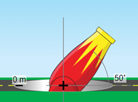
\includegraphics{cannon.png} 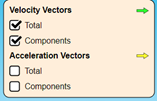
\includegraphics{checkboxes.png}

\end{itemize}







\begin{questions}
  \question
    Describe the shape of the trajectory made by the projectile.\vs

  \question
    Look back at your notes.  What is meant by the terms `$x$-component' and `$y$-component'?  Label on the picture below which one is which.

    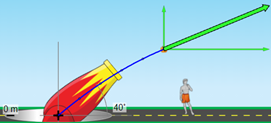
\includegraphics{xy.png}
    \vspace{2em}

  \question
    When you fire the cannon, what happens to the $x$-component of the vector over time? \vs
    
    
  \question
    When you fire the cannon, what happens to the $y$-component of the vector over time? \vs


    
  \question
    On the simulation, increase and decrease the initial speed. How are the range (that is, how far across the ground) and height (that is how far in the air) affected by changing the initial speed? Why do you think this is? \vs
    
  \pagebreak

  \question
    Change from a pumpkin to a tank shell.  The mass of the tank shell is much larger.  

    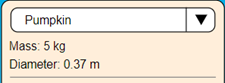
\includegraphics{pumpkin.png} 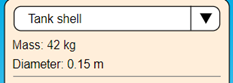
\includegraphics{tankshell.png}
      
    What happens to the trajectory when you use this larger mass?  Why does this make sense? \vs[2]
    
   \question
    Now, keep the initial speed constant but change the angle.  Figure out which angle gives the projectile the tallest height.
    
    \begin{parts}
      \part Which angle has the tallest height? \vs
      \part Why does this make sense? \vs
    \end{parts}

    \question
    Next, figure out which angle gives the projectile the longest range.

    \begin{parts}
      \part Which angle has the longest range? \vs
      \part 
        Explain why projectiles fired at angles close to the ground (like $25^\circ$) don't go as far as projectiles fired at $40^\circ$, $45^\circ$, or $50^\circ$. \vs
      \part 
        Explain why projectiles fired at very high angles (like $85^\circ$) don't go as far as projectiles fired at $40^\circ$, $45^\circ$, or $50^\circ$. \vs
    \end{parts}
    
    \question 
      Can you figure out pairs of angles that give the same range?  Can you notice a pattern? 

      \vspace{1em}
      \fillin[][3em]$^\circ$ and \fillin[][3em]$^\circ$
      
      \vspace{1em}
      \fillin[][3em]$^\circ$ and \fillin[][3em]$^\circ$

      \vspace{1em}
      \fillin[][3em]$^\circ$ and \fillin[][3em]$^\circ$

\end{questions}





\end{document}